\section{Introduction}
The numerical solution of Compressible Couette Flow is performed in this assignment
using nested shooting method. Couette Flow is one of the benchmark problems used in
the fluid dynamics for the validation of numerical codes developed. The present
problem has analytical solution that has been compared with the numerically
obtained solution for the validation of the code developed. The numerical
solver code was developed using \emph{Python3} general purpose programming
language. The procedure and background theory were obtained from \cite{ref_1}.

\section{Governing equations}
\par The reduced form of equations are obtained from the full Navier-Stokes equaitons
for the Compressible Couette flow, the reduced momentum equation is given in \Cref{u_eqn}.
\begin{align}
    \frac{\partial}{\partial y}\left( \mu \frac{\partial u}{\partial y}\right) = 0 \label{u_eqn}
\end{align}

\par The energy equation is obtained as given below.
\begin{align}
    \frac{\partial}{\partial y}\left(k \frac{\partial T}{\partial y}\right) + \frac{\partial}{\partial y}\left(\mu u \frac{\partial u}{\partial y}\right) &= 0 \nonumber
\end{align}
which can be further simplified by substituting the definition for shear stress, leading to \Cref{t_eqn}.
\begin{align}
    \frac{\partial}{\partial y}\left(k \frac{\partial T}{\partial y}\right) + \tau \frac{\partial u}{\partial y} &= 0 \label{t_eqn}
\end{align}

\par Further, the expression for viscosity is taken as a simplified linear
dependence model of temperature given in \Cref{mu_eqn}.
\begin{align}
    \mu = \mu_0 \left(\frac{T}{T_0}\right) \label{mu_eqn}
\end{align}
\par The reference values are taken as \(\mu_0 = 1.789e-5 \ Pa.s\) and
\(T_0 = 288.16 \ K\).

\par The thermal conductivity is governed using the Prandtl number definition
as given in \Cref{k_eqn}, the gas is taken to be calorically perfec with \(C_p = 1005.0 \ J/kg.K\)
and \(Pr = 0.72\).\\
\begin{align}
    k = \frac{\mu C_p}{Pr} \label{k_eqn}
\end{align}

\par All the parameters were non-dimensionalized with their respective reference
values so that the domain in y-direction varies from 0 to 1. The temperatures
were normalized using $T_0$, viscosity with $\mu_0$, and the thermal conductivity
using $k_0$ which is given by \Cref{k0_eqn}.
\begin{align}
    k_0 = \frac{\mu_0 C_p}{Pr} \label{k0_eqn}.
\end{align}

\par After all the non-dimensionalization process, the final governing equations
obtained are given in \Cref{u_Feqn,t_Feqn}.
\begin{align}
    \frac{\partial}{\partial y^\prime}\left(\mu^\prime \frac{\partial u^{\prime}}{\partial y^\prime}\right) &= 0 \label{u_Feqn} \\
    \frac{\partial}{\partial y^\prime}\left(k^\prime \frac{\partial T^{\prime}}{\partial y^\prime}\right) + Pr Ec \times \tau^\prime\frac{\partial u^\prime}{\partial y^\prime} &= 0 \label{t_Feqn}
\end{align}

\par where, \(Pr Ec = A\) is the product of Prandtl number and Eckert number, the boundary conditions for the scenarios are given in \Cref{bc_ewt,bc_aw}.

\begin{table}
   \centering
    \caption{Boundary conditions for case with equal wall temperatures}
    \label{bc_ewt}
    \begin{tabular}{|c|c|c|}
        \hline
        parameter & at y = 0 & at y = 1 \\ \hline
        u & fixed value, u = 1 & fixed value, u = 0 \\ \hline
        T & fixed value, T = 1 & fixed value, T = 1 \\ \hline
    \end{tabular}
\end{table}

\begin{table}
   \centering
    \caption{Boundary conditions for case with adiabatic top wall}
    \label{bc_aw}
    \begin{tabular}{|c|c|c|}
        \hline
        parameter & at y = 0 & at y = 1 \\ \hline
        u & fixed value, u = 1 & fixed value, u = 0 \\ \hline
        T & fixed value, T = 1 & fixed gradient, \(\frac{\partial T}{\partial y} = 0\) \\ \hline
    \end{tabular}
\end{table}


\section{Numerical procedure}
The well known \emph{shooting} method is used for the solution of the equations. Here,
there are two unknowns, $u, T$, hence the equation for temperature is taken to be
\Cref{t_Feqn} and the one for velocity is taken from the definition of shear stress
given in \Cref{tau_eqn}, as the shear stress for this flow problem is a constant, it
is obtained from \Cref{u_Feqn}.
\begin{align}
    \frac{\partial}{\partial y^\prime} \left(\mu^\prime\frac{\partial u^\prime}{\partial y^\prime}\right) = \frac{\partial \tau^\prime}{\partial y^\prime} = 0 \nonumber \\
    \frac{\tau^\prime}{\mu^\prime} = \frac{\partial u^\prime}{\partial y^\prime} \label{tau_eqn}
\end{align}

\par Upon nondimensionalization, an expression that relates temperature,
viscosity and thermal conductivity in their nondimensional form is given in
\Cref{ktmu_eqn}.
\begin{align}
    T^\prime = \mu^\prime = k^\prime \label{ktmu_eqn}
\end{align}

\par The procedure of solving the equations using shooting method, as given in
\cite{ref_1} is as follows.
\begin{enumerate}
    \item A value for \(\tau\) is assumed in \Cref{t_Feqn} using the incompressible
        definition of shear stress. Also the initial velocity profile is assumed
        to be linear.
    \item starting at \(y=0\) with the known boundary condition of wall temperature,
        \Cref{t_Feqn} is integrated till \(y=1\), using first order Euler method
        of numerical integration, since the equation is second order, two
        boundary conditions are to be specified. Tempeature is fixed at
        lower wall, and the gradient of temperature is assumed to be some value.
    \item After reaching the top wall in integration, the temperature obtained
        at the wall is checked if it matches with the top boundary condition. If not,
        then the initial temperature gradient assumption at bottom wall is
        adjusted and re-integration is performed. Newton-Raphson method is
        implemented for the so called shooting method.
    \item From the converged temperature profile, the variation of non-dimensional
        dynamic viscosity and thermal conductivity can be obtained from
        \Cref{ktmu_eqn}. Using the updated value of \(\mu^\prime\), the \Cref{tau_eqn}
        is numerically itegrated for the new velocity profile, from bottom wall
        till top wall.
    \item The velocity value obtained at the top wall is checked to match with
        the boundary condition, and if it does not match, then the value of
        non-dimensional shear stress (assumed in first step) is adjusted to
        match the velocity profile, a second shooting method is implemented
        for this.

    \item Then the procedure is repeated till both the velocity and temperature
        profiles does not vary significantly between the iterations.
\end{enumerate}

\section{Numerical solution results and validation}
\par The analytical expressions for temperature and velocity profiles for the
case with constant equal wall temperatures are given in \Cref{u_A_ewt_eqn,t_A_ewt_eqn}.
\begin{align}
    y^\prime &= 1 - u^\prime\left(\frac{1 + 0.25 \times A \times u^\prime - \frac{1}{6} Au^{\prime 2}}{1 + \frac{1}{12}A}\right) \label{u_A_ewt_eqn} \\
    T^\prime &= 1 + \frac{1}{2} A u^\prime \left(1 - u^\prime\right) \label{t_A_ewt_eqn}
\end{align}

\par where \(A = Pr. Ec.\). Similarly the analytical expressions for temperature and velocity profiles
for the case with adiabatic top wall and constant temperature bottom wall are
given in \Cref{u_A_aw_eqn,t_A_aw_eqn}.
\begin{align}
    y^\prime &= 1 - u^\prime\left(\frac{1 + 0.5 \times A \times \left(1 - \frac{u^\prime}{2}\right)}{1 + \frac{1}{4}A}\right) \label{u_A_aw_eqn} \\
    T^\prime &= 1 + \frac{1}{2} A \left(1 - u^{\prime 2}\right) \label{t_A_aw_eqn}
\end{align}

\par The numerically computed results were compared with the analytical solutions
given by \Cref{u_A_ewt_eqn,u_A_aw_eqn,t_A_ewt_eqn,t_A_aw_eqn}. The solution
for the case with equal constant wall temperatures is given in \Cref{sol_ewt_u,sol_ewt_t}.

\begin{figure}[!h]
   \centering
    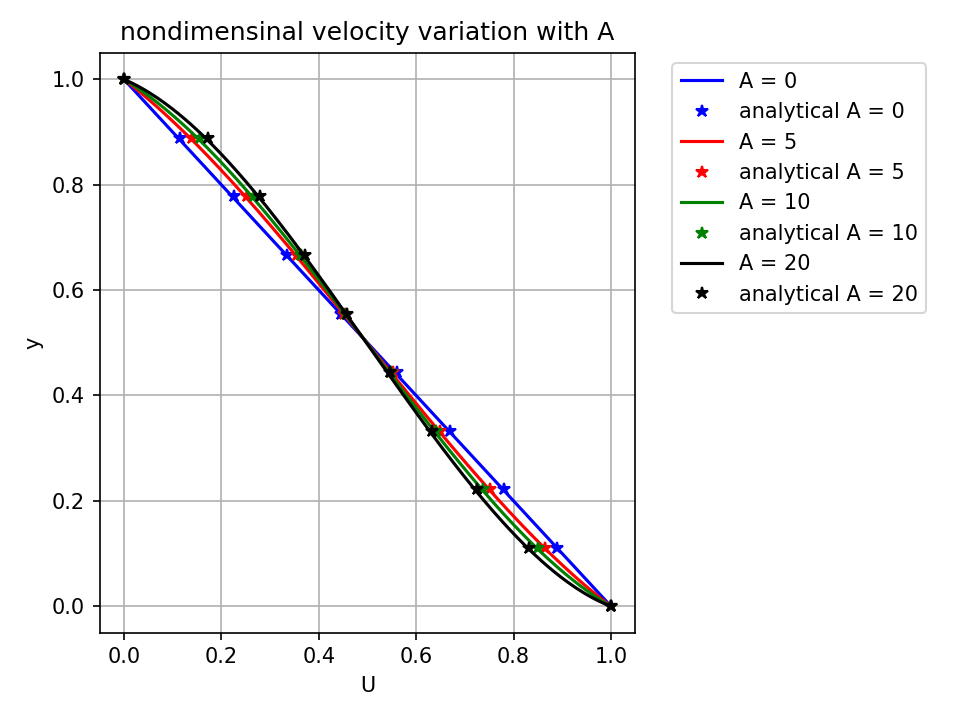
\includegraphics[scale=0.6]{supporting_documents/01_equalWallTemperatures/U_profiles.png}
    \caption{variation of velocity profile for the different values of A, case with equal wall temperatures}
    \label{sol_ewt_u}
\end{figure}

\begin{figure}[!h]
   \centering
    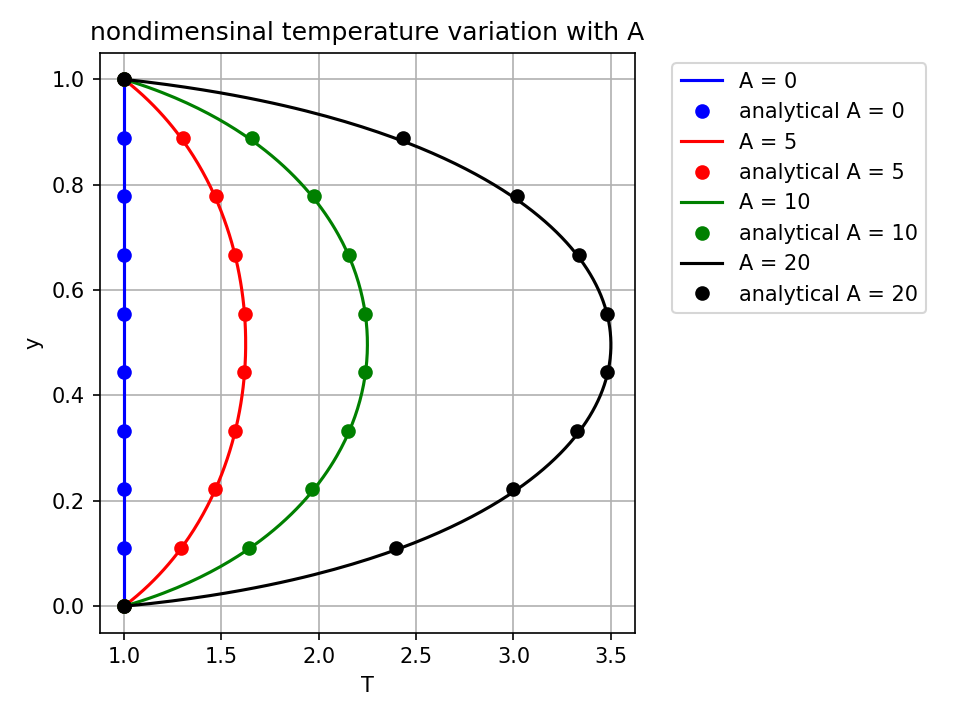
\includegraphics[scale=0.6]{supporting_documents/01_equalWallTemperatures/T_profiles.png}
    \caption{variation of temperature profile for the different values of A, case with equal wall temperatures}
    \label{sol_ewt_t}
\end{figure}

\par Similarly, the numerically computed results for the case with adiabatic
top wall were compared against the analytical solutions and are given in
\Cref{sol_aw_u,sol_aw_t}.

\begin{figure}[!h]
   \centering
    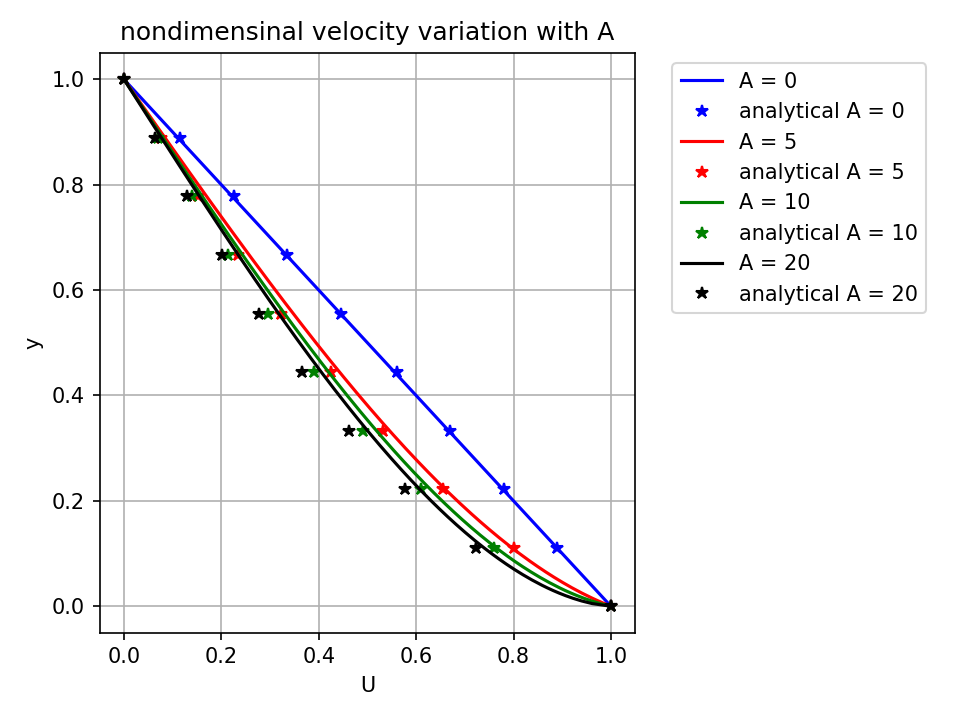
\includegraphics[scale=0.6]{supporting_documents/02_adiabaticWall/U_profiles.png}
    \caption{variation of velocity profile for the different values of A, case with adiabatic top wall}
    \label{sol_aw_u}
\end{figure}

\begin{figure}[!h]
   \centering
    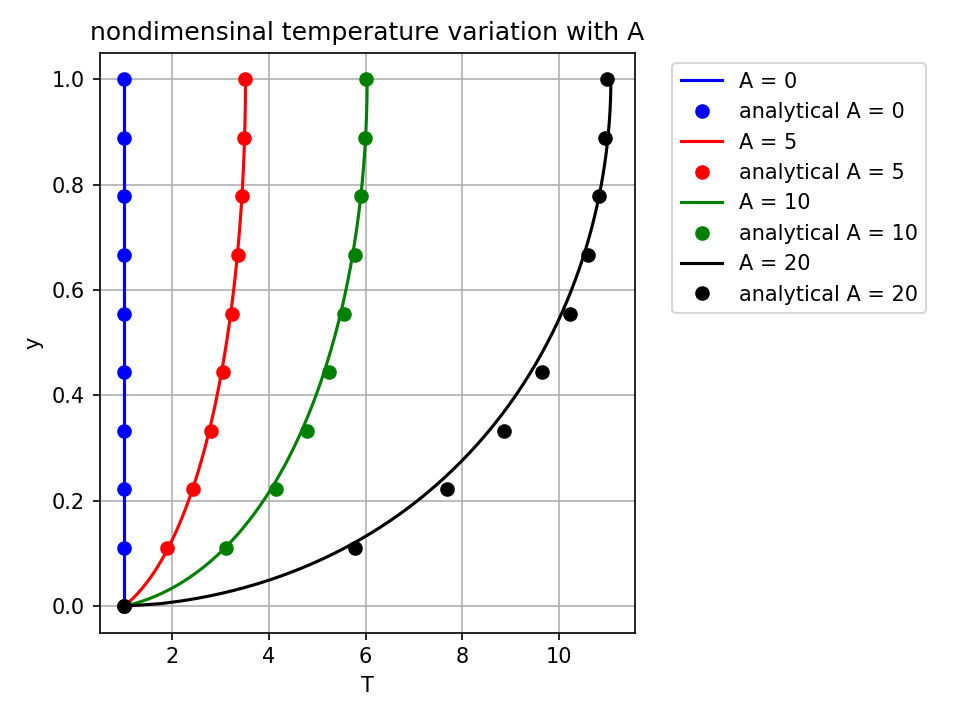
\includegraphics[scale=0.6]{supporting_documents/02_adiabaticWall/T_profiles.png}
    \caption{variation of temperature profile for the different values of A, case with adiabatic top wall}
    \label{sol_aw_t}
\end{figure}

From \Cref{sol_ewt_u,sol_ewt_t,sol_aw_u,sol_aw_t}, it can be noted that the
numerical solution matches well with the analytical solution, hence the
code developed for the solution of these equations is validated.

\pagebreak

\section{Conclusion}
The solution of Compressible Couette Flow has been computed numerically using
nested shooting method with nondimensional governing equations and the results
were compared against the solutions obtained using analytical expressions provided.
Two scenarios were taken, one with equal constant wall temperatures and
the other with adiabatic top wall and bottom wall being with constant
temperature. The code developed for this assignment is validated against the
analytical solution and are given in \Cref{ewt_code,aw_code}.
